%
%  Vincent Yannello
%
\documentclass[12pt,fullpage]{article}
\usepackage{fullpage}
\usepackage{amsmath}
\DeclareMathOperator{\erf}{erf}
\usepackage{psfrag}                                          % LaTeX graphics tool
\usepackage{pslatex}                                         % avoids the default cmr font
\usepackage{graphicx}                                        % graphics package 
\usepackage{epsfig}                                          % figures
\usepackage{hyperref}
\usepackage{color}

\begin{document}

\noindent
{\bf Negative hypergeometric distribution} (from \color{blue}\url{http://www.math.wm.edu/~leemis/chart/UDR/UDR.html}\color{black})

\noindent
The shorthand $X \sim {\rm negative\  hypergeometric}(n_1,\, n_2,\, n_3)$ is used to indicate that the
random variable $X$ has the negative hypergeometric distribution with parameters $n_1$, $n_2$, and $n_3$.
A negative hypergeometric random variable $X$ with parameters $n_1$, $n_2$, and $n_3$ has probability mass function 
$$
f(x) = {\frac {{n_1 + x - 1\choose x} {n_3 - n_1 + n_2 - x - 1\choose n_2 - x}}{{n_3 + n_2 - 1\choose n_2}}}
 \quad \quad x = \max\left\{0, n_1 + n_2 - n_3 \right\}, \ldots, n_2
$$
for all $n_1 \in \{ 1, 2, \ldots, n_2 \}$, $n_2, n_3 \in \{ 1, 2, \ldots \}$. The probability mass function for $n_1 = 5, n_2 = 20,$ and $n_3 = 30$ is illustrated below.
\begin{figure}[h!]
\begin{center}
\psfrag{labx}{$x$}
\psfrag{labf}{$f(x)$}
\includegraphics[width=3.6in]{NegativehypergeometricPlot.ps}
\end{center}
\end{figure}


\noindent
The cumulative distribution, survivor function, hazard function, cumulative hazard 
function, and inverse distribution function, moment generating function, and characteristic function
 on the support of $X$ are mathematically intractable.

 \vspace{0.05in}

\noindent
The population mean, and variance of $X$ are
$$
E[X] = \frac{n_1 n_2} {n_3} \qquad \qquad 
V[X] = \frac{n_1 n_2 (n_3 + n_2)} {n_3(n_3 + 1)} \left(1 - \frac{n_1} {n_3}\right) \qquad \qquad 
$$
The skewness, and kurtosis of $X$ are mathematically intractable.\\

\vspace{0.1in}

\newpage
\noindent
{\bf APPL verification:}
The APPL statements
\begin{verbatim}
assume(0 < n1 < n2);
X := [[x -> binomial(n1 + x - 1, x) * binomial(n3 - n1 + n2 - x - 1, n2 - x)
        / (binomial(n3 + n2 - 1, n2))], [0 .. n2], ["Discrete","PDF"]];
Mean(X);
Variance(X);
Skewness(X);
Kurtosis(X);
MGF(X);
\end{verbatim}
return the population mean, variance, skewness, kurtosis, and moment generating function.

\end{document}
